% !TEX root=./proposal.tex

\subsection{研究背景和科学意义}


%0.人工智能技术很广泛,智能软件越来越多进入人们的生活1.于此同时,其安全问题也得
%到越来越多的关注2.当前的研究主要针对单个智能组件研究其脆弱性,如对抗攻击,后门
%攻击等。近年来,逐渐有少量研究深度学习基础包和依赖库的漏洞,然而如何利用第三方
%开源组件漏洞去激活智能组件的脆弱性研究较少。
%举例
%挑战:3点
%本项目的研究意义3点

%
% 0.人工智能技术很广泛,智能软件越来越多进入人们的生活
近年来,在数据和算力的驱动下,深度学习取得了巨大的成功。如\cref{fig:ch1:intro}所示,深度学习通过特征变换和逐层处理,学习
输入数据的特征表示,深度学习模型对复杂问题的解决能力使其研究成果逐渐从实验室走向实际应用,如计算机视觉
~\cite{dai2021up}、语音识别~\cite{baevski2021unsupervised}和机器翻译~\cite{fan2021beyond}等,并开始部署在自动驾驶
~\cite{feng2021review}、智慧医疗~\cite{liang2021accurate}和航空航天~\cite{julian2019deep}等关键任务上。在获得巨大成功的
同时,深度学习模型的错误行为也导致了很多安全事故。2018年3月19日,在美国亚利桑那州,一辆处在自动驾驶状态的Uber撞击一名女
子,致其不幸身亡,同年7月,Uber宣布停止研发自动驾驶货车。这些事故发生的根本原因是现有技术对深度学习模型的可靠性缺乏系统
性测试,这不仅为应用本身埋下了隐患,也阻碍了深度学习技术在安全攸关任务(如\textbf{交通、医疗、军工}等)的应用。因
此,\textbf{迫切需要在部署深度学习模型前找到其潜在的错误行为来提升深度学习在安全攸关任务上的可靠性}。

Szegedy等人~\cite{szegedy2013intriguing}首次发现,数据中微小的扰动,即便无法被人类发现,却可能造成模型做出错误判断,并由
此引发了很多关于对抗攻击的研究~\cite{yuan2021meta}。事实上,部署在真实世界的模型也可能遇到各种各样的自然意外,如天气的改
变、路标损坏等,这些自然对抗样本也可能导致模型做出错误预测~\cite{hendrycks2021natural}。除了鲁棒性,\textbf{模型的泛化能
    力对于其走向实际应用也有极为重要的意义}。深度学习的目标可定义为训练一个模型${f}$,使得该模型能够适用于真实数据分布
$\mathcal D_{gt}$中任意一个从未见过的数据,而不仅仅是记住训练数据。为了提高真实部署的可靠性,需要系统测试深度学习模型的
泛化能力$\gamma_{gt}$:$\mathbb{E}_{(x, y) \sim \mathcal{D}_{g t}} \mathbb{I}[f(x)=y]$。然而,由于客观世界的真实数据分布
是未知的,因此通常在测试集$\mathcal D_{\text{test}}$上评估模型性能$\gamma_{\text {test }}:\left(1 /\left|\mathcal
    D_{\text {test }}\right|\right) \sum_{(x, y) \in \mathcal D_{\text {test }}} \mathbb{I}[f(x)=y]$。若${f}$的泛化能力较
强,则其在足够充分的测试集$\mathcal D_{\text{test}}$上的性能应接近其在真实数据分布$\mathcal D_{gt}$上的性能。因
此,\textbf{针对泛化能力的深度学习模型测试目标}为:
\begin{itemize}
    \item[(1)] 找出使模型做出错误预测的数据$\mathcal D_{\text{failures}}$,即
          $\mathcal D_{\text{failures}}=\{(x, y) | (x, y) \in \mathcal D_{\text{test}}
              \wedge f(x) \neq y\}$;
    \item[(2)] 生成测试数据集$\mathcal{D}_{\text{test}} \sim \mathcal{D}_{\text{gt}}$
          ,以揭示模型在真实数据分布上所期望的性能$\gamma_{gt}$和实际测试集上所表现的
          性能$\gamma_{\text{test}}$之间的差异;
    \item[(3)] 根据测试反馈信息,找到模型在泛化能力上的不足,进一步提升模型性能。
\end{itemize}

\begin{figure}[htp]
    \centering
    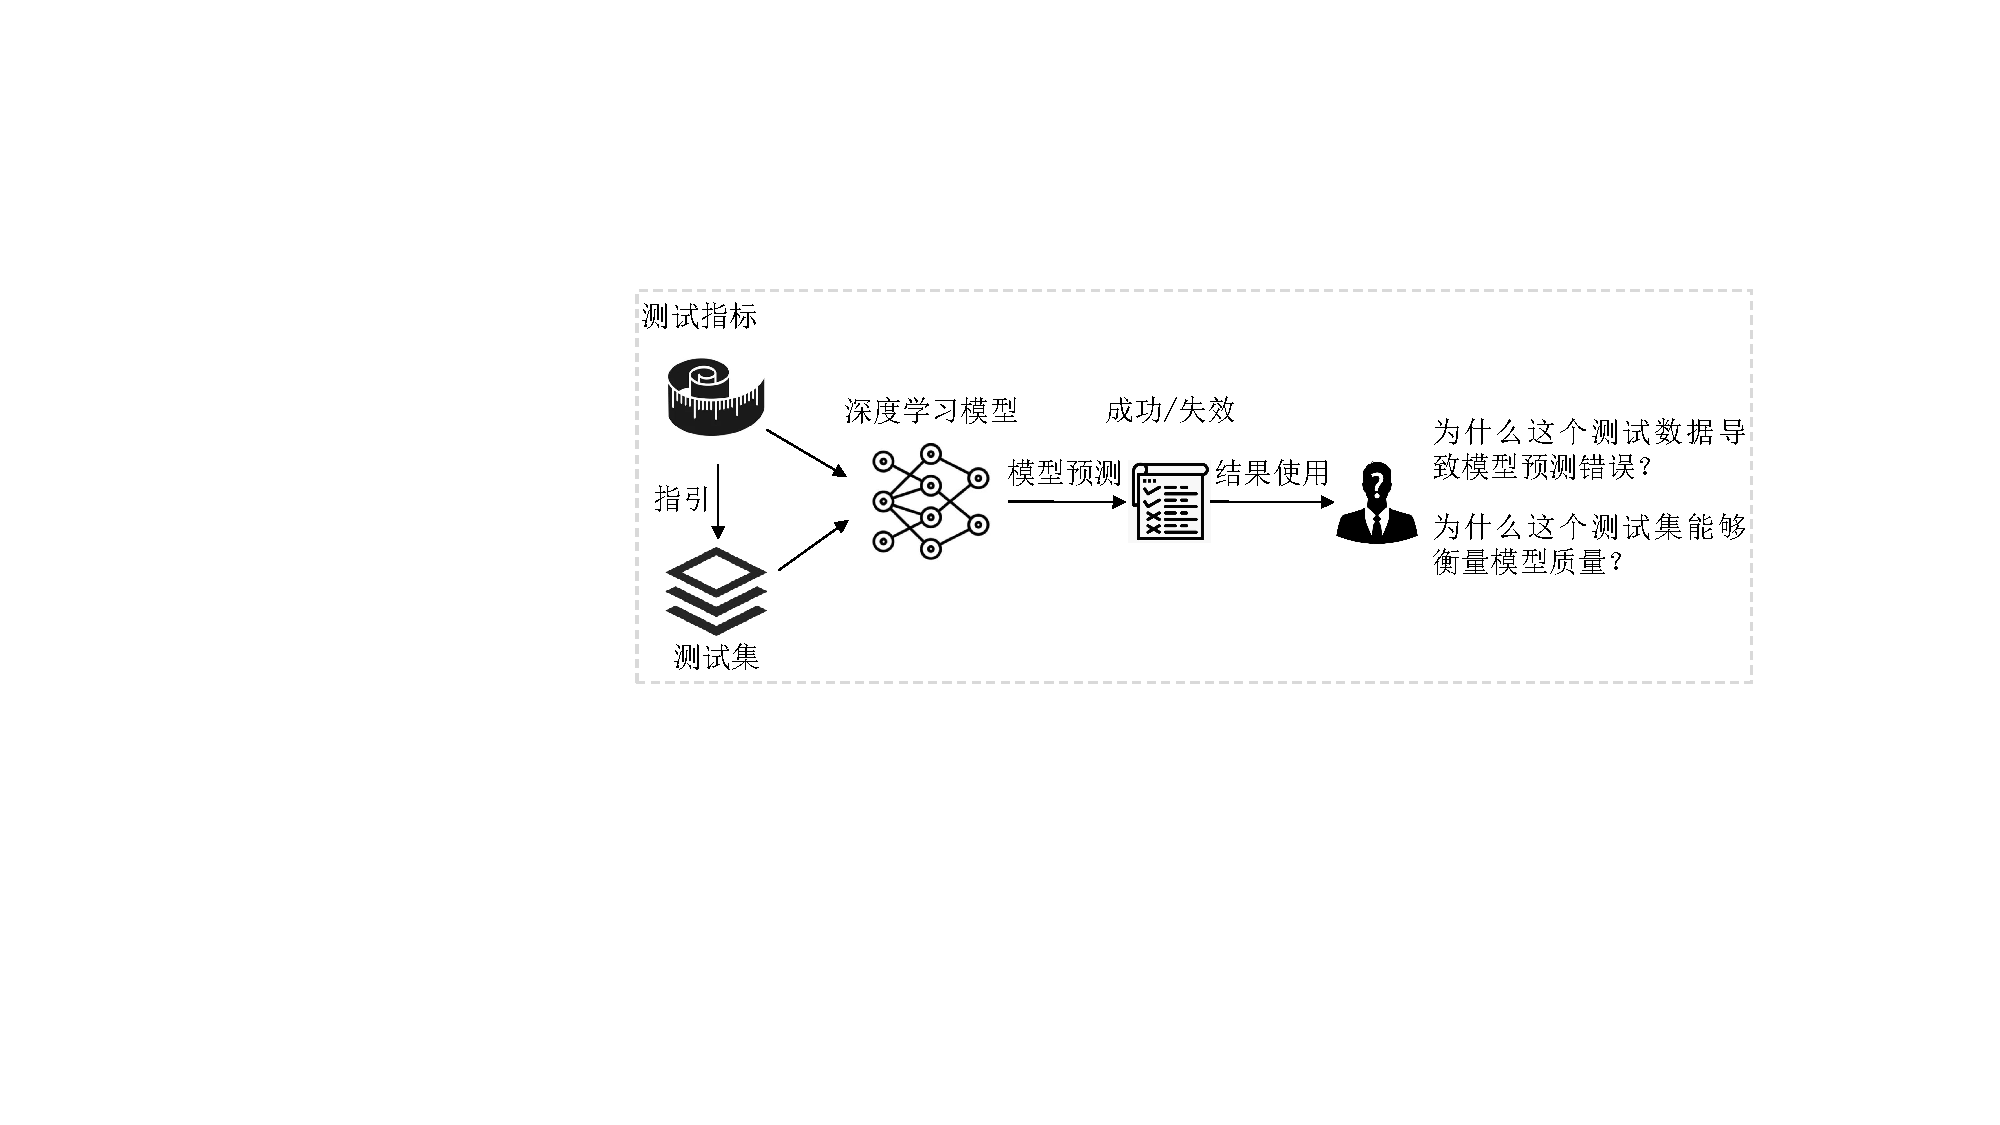
\includegraphics[width=0.8\linewidth]{intro.pdf}
    \caption{深度神经网络测试示意}
    \label{fig:ch1:intro}
\end{figure}

深度神经网络测试(见\cref{fig:ch1:intro})是衡量和改善深度学习模型质量问题的重要手段,已成为助力深度学习技术在安全攸关领
域成功落地的新兴研究热点。如\cref{fig:ch1:intro}所示,给定一个深度神经网络, \textbf{测试度量指标}用于衡量测试集对深度神
经网络的测试充分程度;\textbf{测试输入}指用于测试深度神经网络的输入数据,可分为自然样本和人工样本,通常根据不同的测试度
量指标来指标测试输入生成;除输入数据外,还需\textbf{测试预言}来判断模型在各种输入下的表现是否符合预期。经过系统性测试,
能够获得测试集对深度神经网络的测试充分性、成功/失效执行的测试用例以及模型性能评估结果,最后根据\textbf{测试反馈}指导输
入数据生成,找到更多使模型做出错误决策的测试数据,辅助训练数据扩充和模型修复。

%美国白宫颁布了《维护美国在人工智能领域领导地位》、《国家人工智能研发战略》;欧
%盟致力于打造“从实验室进入市场”,发布《2021人工智能协调计划审查》;俄罗斯发布
%《2030年前国家人工智能发展战略》; 2017年7月,我国国务院印发《新一代人工智能发
%展规划》,旨在构筑我国人工智能发展的先发优势,2019年科技部印发《国家新一代人工
%智能创新发展试验区建设工作指引》,全面提升人工智能创新能力和水平。



%2019年国家新一代人工智能治理专业委员会发布《新一代人工智能治理原则——发展负责任
%的人工智能》,该文件中指出“\textbf{人工智能系统应不断提升透明性、可解释性、可靠
%性、可控性},逐步实现可审核、可监督、可追溯、可信赖”。

% 2. 现有工作和方法的不足
近年来,越来越多的研究致力于深度学习模型的系统性测试。加拿大阿尔伯塔大学的Lei Ma团队深入研究了神经网络测试覆盖
指标~\cite{ma2018deepgauge,ma2019deepct}、测试数据生成~\cite{xie2019coverage,xie2019deephunter}、鲁棒性
~\cite{wang2020deepsonar,sun2020stealthy,zhang2020generating}和模型修复~\cite{yu2021deeprepair}等问题。国内南京大学的陈
振宇老师团队在对话系统~\cite{liu2021dialtest}、医疗~\cite{hou2021taumed}、机器翻译~\cite{ji2021automated}、司法文书
~\cite{guo2020taujud}以及深度学习框架测试~\cite{zhang2021duo,zhang2021predoo,luo2021graph}等领域取得了很好的研究成
果。\textbf{本项目申请人也在自动驾驶软件安全方面提出了针对神经网络模型的测试数据集生成方法~\cite{xu2021deepsuite}}。虽然
已有研究在测试度量指标构建、测试输入生成和测试预言生成等方面已取得一定研究成果,但受传统结构覆盖测试的影响,\textbf{现有
    研究主要集中于对以神经元为基本单位的神经网络架构进行结构覆盖测试},从神经网络和传统软件的主要区别以及深度学习模型测试的
实际需求两方面考虑,现有研究主要存在以下问题:

\textbf{(1)测试指标伸缩性差,难以适用于大规模深度学习模型}

随着数据和算力的发展,深度学习模型的规模近年来呈越来越大的趋势,很多研究证明了大
规模模型对复杂问题的解决能力~\cite{kenton2019bert,he2021masked}。然而,现有的深
度学习结构覆盖测试指标大多难以适用于大规模深度学习模型,主要体现在以下两个方面:
第一,随着模型复杂度的提高,神经元及其取值组合的数量也随之提高,以神经元为基础结
构的结构覆盖率和测试多样性之间的相关性越来越小,导致结构覆盖率对测试集质量的评估
能力骤减;第二,现有结构覆盖指标的计算复杂度与神经元的个数或训练集的规模呈线性增
长关系,伸缩性较差,难以适用于实际使用的大规模深度学习模型。


\textbf{(2)测试结果缺乏可解释性,难以辅助开发人员修复模型}

面向深度学习模型的系统性测试,不仅要评估深度学习模型在特定测试集上的性能表现,还
需要建立测试结果与模型行为之间的联系,从而辅助开发人员修复提升模型。由于深度学习
模型的黑盒性质,现有的基于神经元的结构覆盖指标不能体现深度学习系统的决策逻辑,缺
乏有效语义。虽然在测试覆盖指标的引导下可以生成测试数据,甚至暴露模型的错误行为,
但与传统软件不同的是,开发人员无法知道这些测试数据的成功或失效执行的原因,导致测
试反馈结果很难辅助开发人员定位模型缺陷,提升模型性能。

\textbf{(3)测试数据的标注成本过高,对测试集效率控制不足}

测试用例由输入数据和预期输出两部分组成。在测试一个深度学习模型时,其输入数据的样
本空间经常较大,而人工标注测试预言的成本较高,因此很难在系统部署前检测每个潜在数
据样本的预测正确性。比如图片分类任务中,输入数据是高维连续的图像数据,而目前对图
像的自动标注研究尚在起步阶段,通常需要人工标注图片的类别作为测试用例的预期输出,
在执行测试用例后,根据模型的输出是否符合预期来判断测试用例的成功与否。与此同时,
深度学习模型的测试对测试集的质量有较高要求,即一方面期望测试集能够尽可能模拟真实
数据的分布,准确评估模型性能,另一方面尽早发现容易导致模型预测错误的测试数据,从
而避免在模型部署后仍然存在大量意外输入,导致模型决策错误。为了在有限标注成本内提
高测试的有效性,需要提高测试集的效率,生成规模可控、高质量的测试集。


% 4. 研究方法
深度学习技术正在潜移默化地改变人们的工作和生活方式,其在自动驾驶、恶意软件检测以
及飞机碰撞避免系统等安全攸关领域部署的核心在于“质量”,而深度学习模型的测试技术是
保障深度学习模型质量的必要手段,在这一背景下,\textbf{本项目针对深度学习模型测试
存在的伸缩性差、缺乏可解释性以及标注成本过高的问题,研究适用于大规模神经网络、兼顾测
试成本和测试质量的可解释测试技术,解决了深度神经网络的黑盒复杂特性给模型测试带来的
挑战,为深度学习模型部署在安全攸关领域提供核心技术支撑。}


\subsection{国内外研究现状及发展动态分析}\label{relatedwork}

% 根据与本项目的相关性,本节从覆盖充分性指标、神经网络测试数据生成、深度学习框架测试以及第三方组件漏洞挖掘四个方面介绍和分析国内外研究现状。

根据与本项目的相关性,本节从覆盖充分性指标体系、测试数据集生成、测试数据集优选、
深度学习测试可解释性和知识蒸馏技术等五个方面介绍和分析国内外研究现状。

%研究现状:
%1.覆盖充分性指标体系--缺点,找不到失效原因,不可解释
%2.测试数据集生成方法--本项目申请人--缺点,仅仅针对神经网络,也就是智能组件
%3.框架测试方法--缺点,忽略了其它第三方组件漏洞,可以攻击框架漏洞,给智能组件带来安全威胁,也可以直接激活智能组件的脆弱性。
%4.第三方组件漏洞挖掘--缺点,单组建非跨组件,更缺少组件对人工智能模型各阶段的影响分析。



\subsubsection{覆盖充分性指标研究}
针对深度神经网络的结构覆盖测试启发自传统软件的白盒测试。对于传统软件,若测试集遍
历了待测软件所有的语句、分支和路径,则在一定程度上表明测试集对软件的功能进行了充
分性测试~\cite{hilton2018large}。对于深度神经网络而言,其本身的高维连续特性导致
测试集很难遍历所有可能的输入空间,为提高测试集多样性,目前有很多研究提出了关于深
度神经网络的结构覆盖指标,从不同角度测试衡量测试集对模型的覆盖充分
性。\cref{tab:coverage_criteria}总结了现有神经网络测试覆盖指标,其中$m$表示训练
集规模,$n$表示神经元个数,$l$表示\textbf{XXX}。根据覆盖思想的不同,可分为以下六
类:

\begin{table}[htp]
	\renewcommand\arraystretch{1.5}
	\small
	\centering
	\caption{现有神经网络覆盖充分性指标}
	\label{tab:coverage_criteria}
	% \begin{tabular}{p{3cm}p{5cm}p{1cm}p{1cm}p{2cm}}
	\begin{tabular}{ccccc}
		\toprule
		\textbf{序号} & \textbf{主要思想} & \textbf{覆盖指标}       & \textbf{复杂度} & \textbf{文献号}                                                  \\
		\midrule
		1             & 基于单个神经元取值  & 神经元覆盖、$k$-多区间覆盖                    & $O(n)$          & \cite{ma2018deepgauge}\cite{Pei2019DeepXplore} \\
		2             & 训练集神经元边界  & 神经元边界覆盖、强激活覆盖                    & $O(nm)$          & \cite{ma2018deepgauge}                                           \\
		3             & 与训练数据分布的距离  & 意外覆盖,平均偏差等                & $O(nm)$         & \cite{Kim2019Guiding}\cite{Tian2019Testing}            \\
		4             & 神经元激活通路覆盖    & 符号-符号覆盖、距离-符号覆盖等 & $O(nl)$ & \cite{Wang2019DeepPath}\cite{Sun2018Testing} \\
		5             & 神经元的状态转换        & 状态级别覆盖、转换级别覆盖                         & $O(n)$          & \cite{Du2018DeepCruiser}                                         \\
		6             & 神经元组合测试    & $t$-way组合稀疏覆盖、密集覆盖等 & $O(n^2)$ & \cite{ma2019deepct} \\
		\bottomrule
	\end{tabular}
\end{table}





%其中涉及到的覆盖指标主要有神经元覆盖率(NC),$k$区间覆盖率(KMNC),重要性驱动覆盖
%(IDC),神经元边界覆盖率(NBC),强神经元覆盖率(SNC),重要神经元覆盖(INC),意外覆
%盖(SC),神经元激活向量距离(NAVD),平均偏差(MD),重要神经元通路覆盖率(INPC),强
%激活通路覆盖率(SAPC),符号-符号覆盖(SSC),距离-符号覆盖(DSC),符号-值覆盖
%(SVC),距离-值覆盖(DVC),状态级别覆盖(BSC),转换级别覆盖(BTC),$t-way$组合稀疏
%%%%覆盖($t-way$ CSC),$t-way$组合密集覆盖($t-way$
%CDC),$(p,t)$完整性覆盖($(p,t)$ C)等指标。

%DeepXplore~\cite{Pei2019DeepXplore}、DeepGauge~\citess{ma2018deepgauge}、IDC~\citess{Gerasimou2020Importance}
%等工作主要围绕神经元覆盖率、K区间覆盖率、重要性驱动覆盖等测试覆盖指标。

\begin{itemize}
	\item \textbf{基于单个神经元取值},受结构覆盖思想启发,部分研究者提出度量神
	      经元被覆盖的程度来评估测试充分性。Pei等人~\cite{Pei2019DeepXplore}首次
	      提出了针对深度学习模型白盒测试指标,即神经元覆盖,将取值高于阈值的神经
	      元视为被激活,并计算被激活神经元的比例。 Ma等人~\cite{ma2018deepgauge}
	      提出了$k$-多区间覆盖指标,基于每个神经元在训练集上的取值范围,将其划分
	      为多个取值区间,并计算对神经元值区间的覆盖率。
	      %Gerasimou等人~\citess{Gerasimou2020Importance}设计了通过衡量神经元对分类结果的影响比例提出了重要性驱动覆盖标准。

	\item \textbf{基于训练集神经元的值边界},Ma等人~\cite{ma2018deepgauge}提出神
	经元边界覆盖指标和强激活覆盖指标,计算测试集中神经元的值超过训练集的上下边界
	的比例。

	\item \textbf{基于神经元激活值分布},Kim等人~\cite{Kim2019Guiding}提出了“意
	      外”覆盖指标,衡量模型在测试集和训练集中神经元数据分布距离。Tian等人
	      ~\cite{Tian2019Testing}提出白盒测试框架DeepInspect来检测深度神经网络中
	      的混淆和偏差错误。

	\item \textbf{基于神经元激活通路},Wang 等人~\cite{Wang2019DeepPath}提出了一
	      组针对神经网络模型的路径驱动的测试度量指标,能够更好地识别对抗性样本。
	      Sun等人~\cite{Sun2018Testing}提出将传统的MC/DC覆盖标准应用于深度神经网
	      络,并在此基础上采用梯度搜索的方法生成新的测试集。

	\item \textbf{基于神经元状态},Du等人~\cite{Du2018DeepCruiser}针对循环神经网
	      络提出了状态级别和转换级别两种测试覆盖指标,根据覆盖范围反馈生成具有高
	      覆盖率的测试集,并对基于循环神经网络的自动语音识别系统进行检测。

	\item \textbf{基于神经元组合分布},Ma等人~\cite{ma2019deepct}将组合测试应用
	于神经网络,提出了$t$-way组合稀疏覆盖、$t$-way组合密集覆盖和$(p,t)$完整性覆
	盖等指标。
\end{itemize}

测试覆盖指标是衡量测试集对深度学习模型测试充分性的标尺,是深度学习测试
的重要研究问题之一。{\kaishu 现有测试覆盖指标主要聚焦于对神经网络模型的神经元结构的覆盖研
究,缺少对高层次语义表示覆盖的研究,因此缺乏可解释性。另一方面,现有指标伸缩性较
差,其计算时间和指标有效性难以应对实际大规模模型。本项目拟提出基于知识萃取的可解
释测试覆盖指标,将知识蒸馏和知识回顾应用于神经网络模型测试,从而提升测试指标的伸
缩性和可解释性。}


\subsubsection{测试数据生成方法}

为提高深度学习模型的可靠性,使用足够的测试输入对其一般行为和各种边界条件下的行为
进行充分测试是十分必要的。在对深度学习模型的测试中,如何生成更具代表性的和更容易
暴露模型错误行为的测试数据已成为深度学习测试的一个研究重点。如
\cref{tab:testingDataGen}所示,现有测试数据生成方法可分为以下三类:

\begin{table}[htp]
	\renewcommand\arraystretch{1.5}
	\small
	\centering
	\caption{深度学习模型测试数据生成方法总结}
	\label{tab:testingDataGen}
	% \begin{tabular}{cp{5cm}p{2cm}cp{2cm}}
	\begin{tabular}{cccccc}
		\toprule
		\textbf{序号} & \textbf{算法思想} & \textbf{评价方法}               & \textbf{测试数据} & \textbf{文献号}             \\
		\midrule
		1             & 模糊测试          & 测试覆盖率、效率 & 图像、文本 & \cite{Odena2019TensorFuzz}\cite{Guo2018DLFuzz}\cite{xie2019coverage} \\
		2             & 符号执行          & 测试覆盖率、像素重要性等                              & 图像、代码              & \cite{Gopinath2018Symbolic}\cite{Sun2018Concolic} \\
		3             & 对抗样本          & 准确率、失真度、人类对比评价等 & 图像 & \cite{Xiao2018Spatially}\cite{Wicker2018FeatureGuided}\cite{He2018Decision} \\
		\bottomrule
	\end{tabular}
\end{table}


\begin{itemize}
	\item \textbf{基于模糊测试的思想},通过随机或者特定规则将种子输入进行变换,
	生成新的测试数据,观察模型在边界条件下是否会发生错误。Guo等人
	~\cite{Guo2018DLFuzz}首次提出神经网络模糊测试框架DLFuzz,用于指导生成暴露模
	型错误行为的测试数据。Odena等人~\cite{Odena2019TensorFuzz}利用测试覆盖指标指
	导模糊测试。在此基础上,Xie等人~\cite{xie2019coverage}提出了一个自动化模糊测
	试框架DeepHunter,使用6种测试覆盖指标实现了在深度学习模型开发和部署两个阶段
	的自动化测试。

	\item \textbf{基于符号执行},Sun等人~\cite{Sun2018Concolic}在测试覆盖指标的
	基础上提出了DeepConcolic,结合具体执行和符号分析,提高神经网络的测试覆盖
	率。Gopinath等人~\cite{Gopinath2018Symbolic}提出了一种轻量级符号执行技术并将
	其应用于图像分类算法的测试,以解决重要像素的识别以及创建1像素和2像素攻击等关
	键问题。

	\item \textbf{基于对抗样本的方法},通过向原始样本添加微小扰动的方式产生对抗
	      样本,使深度学习模型做出错误预测。在白盒攻击方面,Xiao等人
	      ~\cite{Xiao2018Spatially}提出了基于空间变换的图像对抗样本生成方法。He
	      等人~\cite{He2018Decision}提出了一种针对区域分类的对抗样本生成方法。在
	      黑盒攻击方面,Wicker等人~\cite{Wicker2018FeatureGuided}提出一种特征引
	      导的鲁棒性测试方法,通过双方博弈游戏的方式确定特征和操作像素点,并利用
	      蒙特卡罗树搜索算法逐步探索博弈状态空间来生成对抗性样本。
\end{itemize}


在深度学习模型部署前找到容易导致模型错误行为的输入数据是必要的。现有测试数据生成
方法主要分为两类:一类受传统软件测试方法启发,在输入种子数据的基础上允许在语义大
致不变的前提下对输入进行变异,以提高覆盖率为导向生成新数据;另一类基于对抗样本,
通过基于梯度等方法搜索导致模型错误预测的最小扰动,生成新测试数据。{\kaishu 然
而,由于神经网络的黑盒特性,这两类测试数据生成方法虽然能够暴露模型错误行为,但测
试结果缺乏可解释性,测试人员很难掌握测试成功或失效的原因,因此除扩充训练集外,对
模型修复的作用较少。本项目拟提出具有可解释性的深度学习模型测试框架,从模型和测试
数据两个角度提高深度学习测试的可解释性。}













\subsubsection{测试数据选择方法}

由于深度学习模型的输入数据的样本空间通常较大,而人工标注测试预言的成本较高,因此
很难在系统部署前检测每个潜在数据样本的预测正确性。为解决这个问题,部分研究提出测
试数据选择方法,从大规模无标注数据中选择出优先标注和测试的输入数
据。\cref{tab:testingDataPri}总结了现有测试数据选择方法,根据选择思想的不同可分
为以下三类:

\begin{table}[htp]
	\renewcommand\arraystretch{1.5}
	\small
	\centering
	\caption{深度学习模型测试数据集优选方法总结}
	\label{tab:testingDataPri}
	\begin{tabular}{cccc}
		\toprule
		\textbf{序号} & \textbf{算法思想}  & \textbf{测试对象} & \textbf{文献号}                                                    \\
		\midrule
		1             & 采用变异测试的思想       & 图像              & \cite{Wang2021Prioritizing}\cite{Ma2018DeepMutation}  \cite{Liu2022DeepState}                    \\
		2             & 基于测试数据的执行结果       & 图像、自然语言  & \cite{Byun2019Input}\cite{Shen2020MultipleBoundary}\cite{Feng2020DeepGini}\cite{Hu2022AnEmpirical}\cite{Gao2022Adaptive} \\
		\bottomrule
	\end{tabular}
\end{table}

\begin{itemize}

	\item \textbf{基于变异测试的思想},部分研究对神经网络模型进行变异,优选能够
	      检测出较多变异模型的测试数据进行标注。Ma等人
	      ~\citess{Ma2018DeepMutation}从训练数据、训练代码和深度学习模型三个角度
	      注入错误,通过错误检出率衡量测试数据质量。Wang等人
	      ~\citess{Wang2021Prioritizing}利用learning-to-rank算法
	      ~\citess{liu2019exploiting}构建测试数据排序模型,能够针对不同的深度学
	      习模型自动优选具有较高错误检测能力的测试数据。Liu等人
	      ~\citess{Liu2022DeepState}提出一种针对循环神经网络的测试集优选方法
	      DeepState,通过捕获神经元状态的变化来识别可能预测错误的测试数据。  

	\item \textbf{基于测试数据的执行结果}, Byun等人~\citess{Byun2019Input}从置
	      信度、不确定性和意外度等三个指标衡量测试数据的错误检测能力,并评估测试
	      数据对于模型再训练的提升。Feng等人~\citess{Feng2020DeepGini}提出一种基
	      于数据统计的测试集优选方法DeepGini,通过输出概率分布识别可能被错误分类
	      的测试数据。Shen等人~\citess{Shen2020MultipleBoundary}将测试数据聚类到
	      深度学习模型的多个边界区域中,从边界区域中均匀选择样本以确保每个边界都
	      有足够的测试数据。Hu等人~\citess{Hu2022AnEmpirical}提出了面向测试集优
	      选的数据分布敏感指标,用来减轻数据分布差异对标注数据集选择的影响。

\end{itemize}

{\kaishu 现有针对深度学习模型的测试数据集优选方法,主要集中于测试数据是否能够反
映模型错误行为,而对测试数据导致模型错误的原因缺乏研究。本项目拟提出基于反馈偏置
的自适应测试集生成,在可解释测试覆盖度量的基础上,选取代表性的样本来解释模型结
果,估算模型性能;同时,自适应找到导致模型错误行为的测试数据优先标注,提高测试集效率。}










\subsubsection{深度学习测试可解释性}

\iffalse
	Zhang等人~\citess{zhang2021duo}提出了一种结合模糊测试和差分生成输入的深度学习框架测试方法Duo,用于解释和评估TensorFlow、PyTorch、MNN、MXNet等深度学习框架;也提出了一种基于模糊测试的算子级精度测试方法Predoo~\citess{zhang2021predoo},用于估计TensorFlow中单个深度学习算子的精度误差。
	Hu等人~\citess{Hu2019DeepMutationPlusPlus}提出了一种基于变异测试的DNN工具DeepMutation++,用于对包括前馈神经网络(FNN)和有状态循环神经网络(RNN)在内的DNN的质量评估,不仅可以静态分析DNN模型对整个输入的鲁棒性,还可以通过运行时分析识别顺序输入的易受攻击部分。
	Xie等人~\citess{Xie2019DiffChaser}提出了一种自动黑盒测试框架DiffChaser,用于检测深度学习模型在量化、压缩前后的非目标或目标不一致性。
	Du等人~\citess{Du2020Marble}提出了的方法Marble构建了一个概率模型,通过抽象来紧凑表征RNN的鲁棒性,用于对基于RNN的深度学习系统进行定量的鲁棒性分析。

	Luo等人~\citess{luo2021graph}将算子级别的覆盖指标引入图论,提出了一种基于图的模糊测试方法来捕捉深度学习框架异常、提高深度学习框架质量和可解释性的方法。
	Du等人~\citess{Du2019DeepStellar}~\citess{Du2019AQuantitative}提出了一个基于对抗性样本检测和覆盖引导测试生成的深度学习模型测试方法DeepStellar,基于两个轨迹相似性指标和五个覆盖充分性指标对循环神经网络(RNN)进行定量分析和可解释性研究。
	Lee等人~\citess{Lee2020Effective}提出了一种对神经网络进行白盒测试的新方法Adapt,通过使神经元选择策略不断地自适应正在进行的测试状态,增强了深度神经网络的可解释性,在覆盖率和对抗性输入方面有有效表现。
	Wang等人~\citess{wang2020deepsonar}提出一种识别AI合成假声音的方法DeepSonar,利用对分层神经元激活模式学习来增强深度神经网络在语音识别方面的可解释性,推测真实和AI合成的假声音之间的细微差异,同时也对操纵攻击(例如语音转换和附加现实世界噪声)的情况具有鲁棒性。
\fi



由于深度学习模型的黑盒特性,开发人员很难将测试结果与模型行为联系起来,深度学习测
试能够提供的有效修复信息较少。目前关于可解释性的研究工作主要集中于深度学习模型本
身的可解释性,而对测试结果的可解释性研究较少。Xie等人~\citess{Xie2021NPC}提出了
神经元路径覆盖指标,类似于传统的程序控制流图,首先从深度神经网络中提取决策图用来
表示模型的决策逻辑,然后基于决策图的控制流和数据流,该方法提出了两种路径覆盖的变
体来衡量测试数据在执行决策逻辑时的充分性。该测试方法在一定程度上反映出模型的决策
逻辑,但由于模型本身缺乏可解释性,难以从控制流或数据流路径上辅助开发人员找到模型
失效的原因,从而帮助修复模型。此外,Chen等人~\citess{Chen2020Practical}提出了一
种可解释的测试数据选择方法,利用基于实例的可解释算法MMD-critic选取具代表性的测试
输入来估算模型在整个测试集上的准确性。该方法的可解释性主要体现在测试数据的选择流
程上,而对测试反馈的可解释性仍然不足。

{\kaishu 虽然结构覆盖测试能够在一定程度上提高测试集的充分性,但由于模型本身的黑
盒特性,现有的深度学习模型测试工作也缺乏可解释性,开发人员很难建立测试结果与模型
行为之间的联系。本项目拟提出针对深度学习模型的可解释测试框架,采用知识蒸馏和知识
回顾的思想,从白盒和黑盒两个角度分别提出可解释测试覆盖指标,通过测试反馈辅助开发
人员修复模型。}

%然而在现实情形中,智能软件大量依赖基础库和第三方依赖库,其脆弱性来源包括智能组件脆弱性、非智能组件脆弱性以及跨组件脆弱性,而智能组件、基础框架组件以及其它第三方组件之间的交互影响尚不明确,第三方开源组件数量极大,版本较多,更新频繁,组件间依赖关系复杂,挖掘可能存在漏洞的脆弱组件难度较大。



\subsubsection{知识蒸馏技术}

知识蒸馏是指一种教师-学生(Teacher-Student)模型训练结构,其目标是以尽可能小的代
价将教师模型学到的知识迁移到简单的学生模型中~\citess{Gou2021KnowledgeDA}。该技术
被广泛应用于模型压缩,目前在图像、文本、音频等多种模态数据的处理任务中均有应用。
在计算机视觉方面,Hou等人~\citess{Hou2020CVPR}通过传输图像样本中不同区域之间的结
构关系,将教师网络学习到的场景结构知识迁移给学生执行道路标记分割任务。Fu等人
~\citess{Fu2020Ultrafast}提出将教师模型学习到的空间和时间知识迁移到低分辨率的轻
量级时空网络中来执行视频注意预测任务,高分辨率数据上训练得到的知识在低分辨率图片
处理任务上具有重要价值,同时能够降低对于计算机资源和存储的要求。在自然语言处理方
面,Wang等人~\citess{Wang2020StructureLevelKD}和Mukherjee等人
~\citess{Mukherjee2020XtremeDistilMD}将若干单语言的教师模型学习到的结构知识和内
部特征迁移到统一的多语言学生模型,来得到轻量级的多语言序列标注模型,而且其性能表
现比原有复杂模型更优。在语音识别领域,Aguilar等人
~\citess{Aguilar2020KnowledgeDF}提出将教师网络的多个Transformer层的特征知识压缩
到学生的单个Transformer层中,Liu等人~\citess{Liu2019EndtoEndST}提出引入自适应层
来压缩Transformer结构,在保持transformer对长序列学习问题的优越性的同时,也减轻了
它过大的参数规模,便于计算和存储。

部分研究将知识蒸馏用于生成具有可解释性的学生模型。Liu等人
~\citess{Liu2018ImprovingTI}将深度神经网络提炼并表示成决策树,将已有问题转化为多
输出回归问题,可以同时获得良好的性能和可解释性。另一方面,知识蒸馏本身也具有一定
的可解释性,从而可以帮助生成可解释的轻量级模型。 Cheng等人
~\citess{Cheng2020ExplainingKD}通过对深度神经网络中间层的量化和分析,提出了对知
识蒸馏所得学生模型性能优越的解释,认为知识蒸馏能够学习到更多的视觉概念。此
外,Phuong等人~\citess{Phuong2019TowardsUK}通过研究线性和深度线性分类器,提出了
蒸馏成功的三个关键原因:一是数据分布的几何特性,二是优化偏差,梯度下降优化找到对
蒸馏目标的非常有利的极小值,三是强单调性,即当训练集的大小增加时,学生分类器的预
期风险总是降低。


{\kaishu 目前知识蒸馏技术已被广泛应用于模型压缩,本项目拟利用部分知识蒸馏技术对
深度学习模型可解释性的提升,融合Kolmogorov-Smirnov检验、D检验等方法构建具有可解
释性的测试覆盖指标,总结归纳模型错误行为的原因,指导训练数据集扩充和模型优化。}








% 因为写 demo,我把参考文献放这里了,真写本子的时候,还是要放在国内外概况那边
\begin{spacing}{1.3} % 行距
	\zihao{5} \songti
	\bibliographystyle{gbt7714-nsfc}
	\bibliography{ref,cai_refs}
	\vspace{11bp}
\end{spacing}
